\section{Anotación}

Hasta este momento describimos la recolección de los datos, proceso al cual le siguió la selección de los artículos y comentarios a anotar. Pasamos ahora a detallar el etiquetado del dataset, describiendo el modelo utilizado (¿qué queremos etiquetar?), el proceso de selección de etiquetadores y las herramientas utilizadas para este fin.


\subsection{Modelo de etiquetado}


Un modelo de anotación es una representación práctica del objetivo de anotación; es decir, del fenómeno que queremos capturar \cite{pustejovsky2012natural}. En base a la discusión del capítulo anterior, es de interés marcar comentarios discriminatorios de manera granular de modo de tener información de qué grupos y/o características se está ofendiendo. Para identificar formas más graves de discurso de odio, también es de interés identificar llamados a tomar alguna acción (violenta o no violenta) contra esa persona o grupo.

\begin{figure}
    \centering
    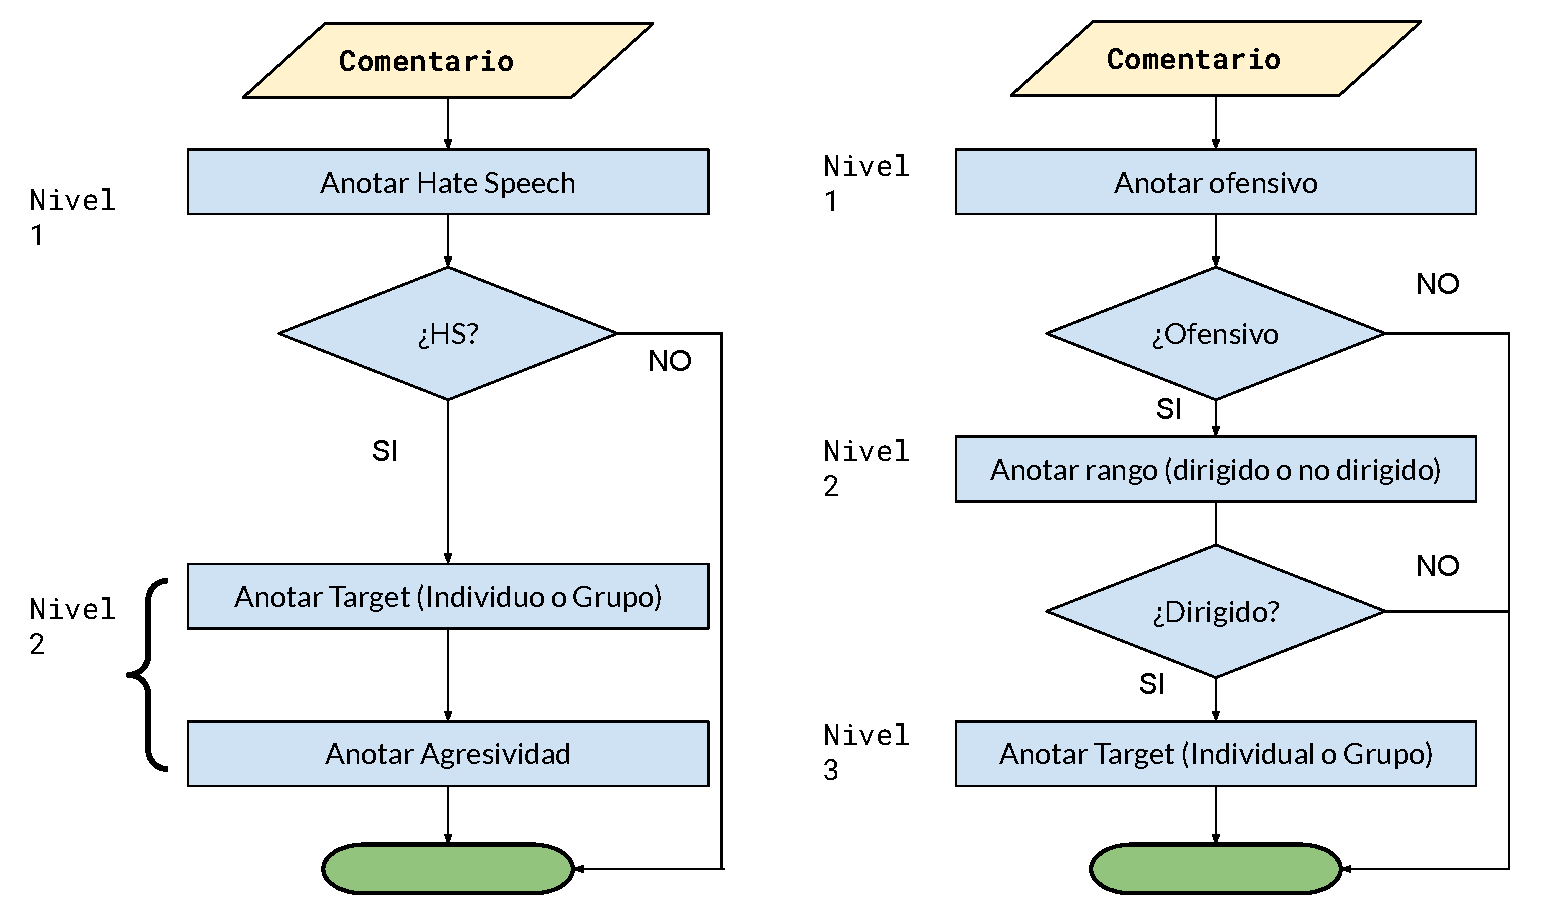
\includegraphics[width=\textwidth]{img/05/modelos_jerarquicos.pdf}
    \caption{Modelos jerárquicos de anotación. A la izquierda, tenemos el modelo jerárquico propuesto para HatEval \cite{hateval2019semeval}, a la derecha el modelo propuesto para OffensEval \cite{zampieri2019semeval2019}}
    \label{fig:modelos_offenseval_hateval}
\end{figure}


\citet{zampieri2019predicting} introdujeron un modelo jerárquico de anotación para la tarea de lenguaje ofensivo, utilizado tanto en los datasets de OffensEval \cite{zampieri2019semeval2019} y HatEval \cite{hateval2019semeval}. La idea de este modelo es realizar anotaciones en varios niveles, sólo marcando algunas variables de acuerdo a las respuestas del nivel predecesor. Por ejemplo, en el caso de \hateval{}, tenemos un primer nivel que consta de marcar si un tweet contiene o no discurso de odio. Si el tweet tiene discurso de odio, entonces se anota en primer lugar si está dirigido a un individuo o a un grupo, y también si es agresivo o no. En el caso de \emph{OffensEval}, primero se anota si es ofensivo, en caso de ser ofensivo se marca si está dirigido o es un insulto no dirigido, y finalmente, si es dirigido y ofensivo, marcamos si su objetivo es un grupo o un individuo.  La Figura \ref{fig:modelos_offenseval_hateval} ilustra en modo de diagrama de flujo el modelo de anotación de ambos conjuntos de datos.


%
%
% Link: https://docs.google.com/drawings/d/14TKSC4QmZhksnlFvQcHUaZup-q3AL0Up1cNKJUr5toI/edit
%



\begin{figure}
    \centering
    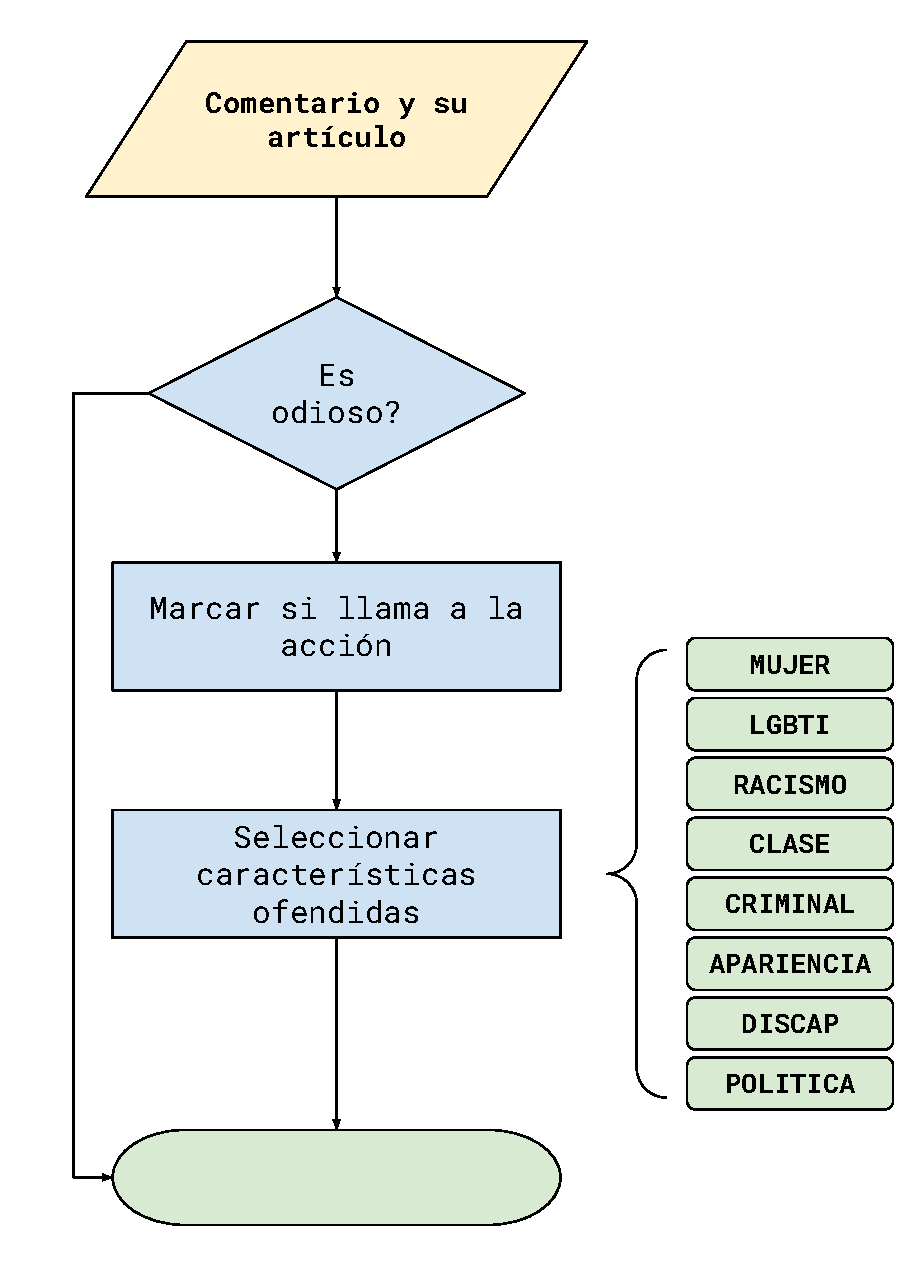
\includegraphics[width=0.5\textwidth]{img/05/annotation_model.pdf}
    \caption{Modelo de anotación para el dataset construido en este capítulo. El modelo jerárquico consta de dos niveles: el primero, donde se anota si es odioso. El segundo consta de anotar --en caso de haber sido marcado como odioso-- si contiene un llamado a la acción y a qué características ofende.}
    \label{fig:annotation_model}
\end{figure}


Basándonos en esta estructura jerárquica planteamos nuestro modelo, ilustrado en la Figura \ref{fig:annotation_model}. Para cada comentario y su respectivo contexto (el artículo), requerimos una anotación para decidir si el comentario es odioso o no. Si no es odioso, no se necesita más información. En caso de haberse marcado como odioso, el par artículo-comentario debe contener, además, una anotación por si llama o no a la acción, y al menos una categoría protegida marcada como ofendida.


\subsection{Definición de discurso de odio y manual de etiquetado}
\label{sec:05_hate_speech_definition}
\begin{table}[t]
    \centering
    \small
    \begin{tabularx}{\textwidth}{l X}
        Nombre & Descripción \\
        \hline
        MUJER        & Misoginia, agresiones basadas en ser mujer  \\
        LGBTI        & Homofobia, transfobia, y ofensas a la comunidad LGBTI \\
        RACISMO      & Racismo, Xenofobia, Judeofobia, etc \\
        POBREZA      & Basado en su condición de clase \\
        POLITICA     & En base a la filiación política del agredido \\
        ASPECTO      & Gordofobia, gerontofobia \\
        CRIMINAL     & Criminales, presos, y personas en conflicto con la ley \\
        DISCAPACIDAD & Discapacidades y problemas de adicciones \\
        \hline
    \end{tabularx}
    \caption{Características protegidas consideradas en este trabajo. Consideramos una agrupación de ciertas características bajo una misma denominación: por ejemplo, LGBTI contempla homofobia, transfobia, entre otras; análogamente racismo puede contemplar xenofobia, y otras variantes de este fenómeno. }
    \label{tab:caracteristicas_protegidas}
\end{table}


Teniendo en cuenta la discusión realizada en la sección \ref{sec:hate_speech_definitions} realizamos nuestra propia definición de discurso de odio. Entendemos que hay discurso de odio en un texto social si éste contiene declaraciones de carácter intenso e irracional de rechazo, enemistad y aborrecimiento contra un individuo o contra un grupo, siendo estos objetivos de estas expresiones por poseer (o aparentar poseer) una característica protegida. Esta expresión puede manifestarse de manera explícita como insultos directos, celebraciones de crímenes, incitaciones a tomar medidas contra el individuo o grupo, o también expresiones más veladas. Siempre, considerando, que no es necesario solamente un insulto o una agresión: es necesario hacer una apelación explícita o implícita a al menos una característica protegida.

A diferencia de otros trabajos, nuestra definición comprende varias características, incluso algunas que están en la frontera de ser ``protegidas''. Mientras en otros trabajos se centran mayormente en racismo y misoginia, aquí agregaremos homofobia y transfobia, odio de clase (a veces conocido como aporofobia), por su aspecto físico, y otras. En particular, hay dos características no convencionales que tuvimos en cuenta. En primer lugar, el discurso de odio ``político'', que de acuerdo a \citet{CIDH2015} (ver sección \ref{sec:hate_speech_definitions}) es difícil considerar como protegida ya que puede dar lugar a censura y restricciones de la libertad de expresión.

Por otro lado, consideramos el discurso de odio contra criminales, presos, y otras personas en situación de conflicto con la ley. Si bien este punto ni siquiera es considerado como una característica protegida en ninguno de los trabajos mencionados en la sección \ref{sec:hate_speech_definitions}, agregamos esta característica debido a la enorme cantidad de contenido alentando la violencia contra criminales en las noticias de policiales, teniendo en cuenta que nos interesa detectar la incitación a la violencia.

Tenemos entonces 8 características que agrupan tipos de discurso de odio: contra las mujeres; racismo y xenofobia; contra la comunidad LGBTI; odio de clase; gordofobia, gerontofobia y demás odio por aspecto; por su ideología política; y finalmente contra discapacitados y adictos. Las características en cuestión son listadas en la tabla \ref{tab:caracteristicas_protegidas} junto a nombres de referencia que usaremos en éste y el próximo capítulo.

Con esta definición confeccionamos un manual de etiquetado de referencia para los anotadores. Esta definición y el manual de etiquetado fueron desarrollados iterativamente, primero realizando algunas pruebas de etiquetado entre miembros del equipo y rondas de discusión posterior analizando los ejemplos problemáticos y casos borde. De estas iteraciones logramos ir mejorando el manual, agregándole ejemplos y definiciones, hasta llegar a una versión definitiva. Para cada característica agregamos algunas consideraciones adicionales: por ejemplo, para MUJER no basta con que se insulte a la mujer sino que se apele a algo distintivo de la mujer (``algo que no le diría a un hombre'') y para la característica LGBTI mencionamos particularmente las expresiones de asco, incluyendo en esto a los emojis. En el apéndice \ref{app:manual_criterios_anotacion} puede encontrarse el manual de etiquetado completo entregado a los etiquetadores.


\subsection{Etiquetadores}

%
% Chequear https://docs.google.com/spreadsheets/d/1PaOVw_tKVRvjZIqRl2YKnaNsvX5tHJjjY0CV9PLrc6g/edit?resourcekey#gid=366330815
%

\begin{table}[t]
    \centering
    \small
    \begin{tabularx}{\textwidth}{l l l l l l l l}
        Género& Edad  & Estudios    & Área          & Identificación    & ¿Activista?   & Experiencia\\
        \hline
        F    & 27     & Doctorado*  & Psicología    & Mujer             & No                   & Sí         \\
        NB   & 33     & Grado*      & Artes         & LGBTTIQ           & No                   & No         \\
        F    & 30     & Grado*      & Antropología  & Mujer, LGBTTIQ    & Feminista            & Sí         \\
        M    & 38     & Grado       & Sociología    & No                & No                   & No         \\
        F    & 36     & Doctorado   & Psicología    & Mujer             & No                   & No         \\
        F    & 34     & Grado       & Comunicación  & No                & Migrantes            & No         \\
        \hline
    \end{tabularx}
    \caption{Información sobre los anotadores. En el caso de estudios, * indica en curso. Indentificación se refiere a si se autopercibe como perteneciente de una característica protegida considerada en este trabajo. Experiencia se refiere a haber etiquetado previamente otros datasets. }
    \label{tab:informacion_sobre_anotadores}
\end{table}

A diferencia de otros trabajos (como hatEval \cite{hateval2019semeval}) decidimos garantizar que nuestros anotadores estén más cerca culturalmente al problema en cuestión y también tener mayor control del perfil de estos. El discurso de odio tiene un fuerte componente cultural, muchas veces expresado a través de jerga o expresiones dialectales muy particulares, y relacionado con noticias muy propias de esta región.

Reclutamos etiquetadores hablantes nativos, estudiantes o graduados/as de carreras de ciencias sociales, humanidades o afines -- como ser Psicología, Sociología, Comunicación, Antropología. Algo que particularmente nos interesó fue que no tengan conocimientos de inteligencia artificial, ciencia de datos ni relacionados de manera de no sesgar su tarea. También, que sean usuarios asiduos de redes sociales.

El proceso de reclutamiento constó en una breve entrevista donde corroboramos que sean hablantes nativos, les describimos la tarea mientras le mostrábamos la herramienta de etiquetado. Finalmente, se les solicitó hacer una prueba paga de leer el manual de etiquetado y anotar 10 artículos. Esto lo hicimos para corroborar la calidad de los etiquetadores. No rechazamos ningún etiquetador en este proceso. La tabla \ref{tab:informacion_sobre_anotadores} brinda información desagregada sobre los 6 etiquetadores. Los etiquetadores reclutados tienen un perfil altamente escolarizado, con 2 etiquetadoras con experiencia previa, y siendo 2 activistas.

Luego de la entrevista, se les dio un feedback de su anotación, y se les reasignaron 5 de los artículos seleccionados junto a diez más (15 en total) para su anotación a modo de entrenamiento. Este es el único conjunto de artículos que fue anotado por la totalidad de los seis anotadores. Al finalizar esta etapa, se les brindó un nuevo feedback para ajustar el criterio de anotación, y se procedió a la etapa de anotación del dataset.

\subsection{Esquema de anotación}


%%
%%
%% Link a Google Draw:
%% https://docs.google.com/drawings/d/1esS9tAwpPVydohxd-B-xwVdAaPQRVGAo0MruBrgSKig/edit
%%
%%

\begin{figure}
    \centering
    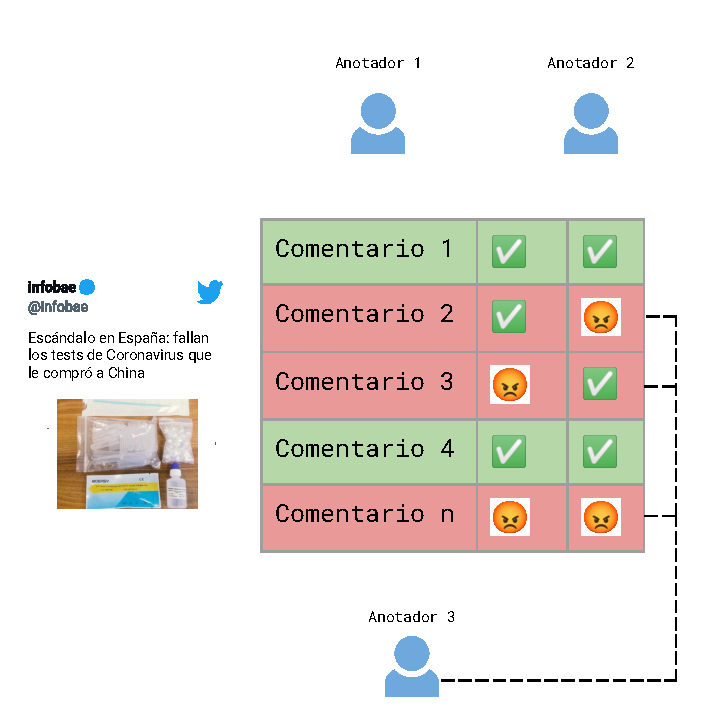
\includegraphics[width=0.7\textwidth]{img/esquema_anotacion.pdf}
    \caption{Esquema de anotación. Caso en que ambos anotadores etiqueten los comentarios del artículo}
    \label{fig:annotation_schema}
\end{figure}

La unidad de anotación del proceso de etiquetado es el artículo. Cada etiquetador, al serle presentado un artículo, tiene dos opciones: etiquetarlo o saltearlo. La idea de saltear es doble: evitar contenido poco ``interesante'' en términos de comentarios discriminatorios, o evitar contenido sensible para el anotador (algo que afortunadamente no ocurrió). En caso de etiquetarlo, tiene que asignarle las etiquetas correspondientes a cada comentario.

Una posibilidad que barajamos en un principio fue asignar el artículo completo a 3 anotadores. Sin embargo, esta modalidad sería altamente ineficiente dada la baja cantidad de contenido discriminatorio. Decidimos entonces ir por un esquema de desempate: dos anotadores anotan un artículo, y luego un tercero anota sólo aquellos donde al menos uno marcó que es discriminatorio. Esto da la posibilidad de que haya una tercera anotación incluso cuando dos previas marcaron que el comentario es discriminatorio, y lo hacemos para recolectar más información. Con este esquema de anotación, y teniendo en cuenta los números finales obtenidos del dataset, dedicamos 2.16 etiquetados por comentarios versus 3 etiquetados por comentario de anotar tres veces todo. La figura \ref{fig:annotation_schema} ilustra este flujo de anotación.


\begin{figure}
    \centering
    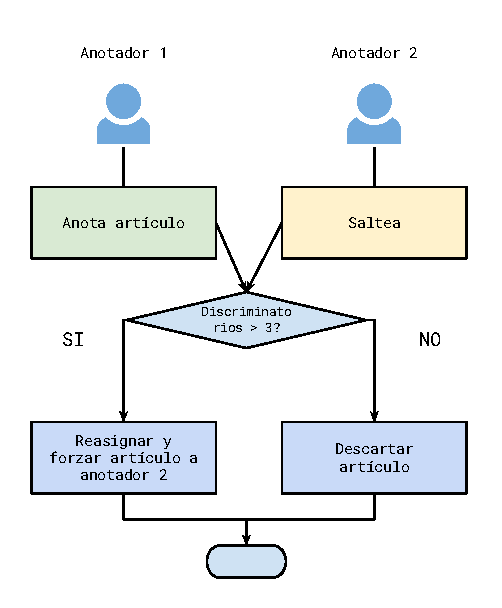
\includegraphics[width=0.4\textwidth]{img/esquema_anotacion_caso_2.pdf}
    \caption{Esquema de anotación. Caso en que un anotador saltee}
    \label{fig:annotation_schema_case_two}
\end{figure}

Cada artículo es, en primer lugar, asignado a 2 anotadores. Luego de esto, se solicita una tercera anotación pero sólo sobre los comentarios que tengan alguna de las dos etiquetas marcando contenido discriminatorio y no dando la posibilidad de saltear a este tercer etiquetador. Ahora ¿qué pasa si alguno de los dos anotadores saltea el artículo?. Tenemos dos casos. Si los dos saltean el artículo, entonces descartamos ese artículo. Ahora, puede ocurrir el caso de que uno lo saltee y el otro lo anote: en ese caso, y en pos de maximizar el contenido discriminatorio encontrado o uno lo hace y el otro anota menos de 4 comentarios odiosos, entonces no pasa a 3ra anotación y lo descartamos del dataset. Si uno salteó y el otro anotador anotó 4 o más comentarios odiosos, entonces forzamos al primer anotador a anotar el artículo, sin dar esta vez opción de saltear. La figura \ref{fig:annotation_schema_case_two} ilustra el flujo para este caso.


Cada tweet es presentado con un preprocesado básico, consistente en reemplazar handles de usuarios por un token especial \verb|@usuario| para evitar cualquier sesgo. Por ejemplo, si un usuario conocido como ``odiador'' (llamemos \verb|@hater|) retwittea la noticia y otro responde a ese RT, aparece ese nombre de usuario lo cual podría condicionar al etiquetador.


%%
%%
%% Link a Google Draw
%% https://docs.google.com/drawings/d/1TOlCgZggCmYHgZWV7ZrIIlXuhcFUMeYw4PcFM7XdY2k/edit
%%
%%


Como resultado de este esquema, cada comentario de nuestro dataset puede tener dos o tres anotaciones, siendo los casos posibles los siguientes:

\begin{enumerate}
    \item Dos anotaciones negativas
    \item Tres anotaciones, siendo al menos una que marque el comentario como discriminatorio
\end{enumerate}


%
% Esto quizás va después
%
\subsection{Herramienta de etiquetado}

%%
%% Link a Google Draw: https://docs.google.com/drawings/d/1E24-2l6hsNj2JSKBZOD8QvZCJR6rrGjz-cWwt8XuPRg/edit
%%

\begin{figure}
    \centering
    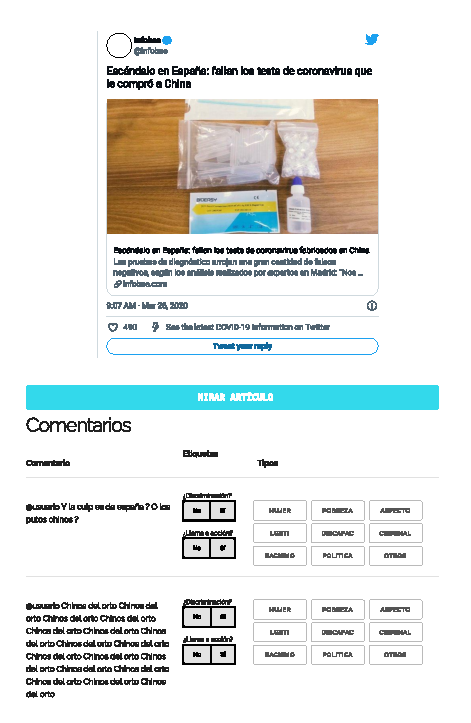
\includegraphics[width=\textwidth]{img/labeler.pdf}
    \caption{Pantalla del etiquetador}
    \label{fig:labeler_example}
\end{figure}

Al no utilizar ningún servicio de etiquetado, optamos por desarrollar nuestra propia aplicación para el etiquetado de tweets. En ella, a cada etiquetador les fueron asignados progresivamente los artículos a anotar, agrupados en ``lotes'' para facilitar la tarea administrativa de la asignación.

La figura \ref{fig:labeler_example} muestra la interfaz presentada a los etiquetadores. Cada artículo es presentado al etiquetador junto a los comentarios asignados. Ante esto, el etiquetador puede elegir saltear el artículo o etiquetarlo. Si decide etiquetarlo, el etiquetador debe para cada comentario marcar usando un control de tipo switch:

\begin{enumerate}
    \item Si el comentario contiene discurso discriminatorio
    \item En caso de ser discriminatorio, marcar si llama a la acción
    \item En caso de ser discriminatorio, marcar al menos una característica ofendida
\end{enumerate}

Para el desarrollo de la aplicación usamos Django\footnote{\url{https://www.djangoproject.com/}}, un framework de python para desarrollo web, y Javascript plano. Como base de datos utilizamos SQLite ya que tenía una baja tasa de concurrencia (sólo 6 usuarios).

\subsection{Asignación}

Llamamos \tbf{asignación} al procedimiento de asignar \tbf{gold labels} al dataset anotado \cite{pustejovsky2012natural}. Nuestro modelo consta de una etiqueta binaria marcando si el contenido es discriminatorio o no (notamos HS) en el primer nivel, y luego 9 etiquetas binarias: una para la llamadas a la acción (CALLS) y otras 8 para las características ofendidas. Recordemos que una anotación negativa sólo consta de HS negativo, mientras que una positiva consta de un HS positivo, una etiqueta para CALLS y al menos una etiqueta positiva de las características restantes.

Para este dataset, tomamos las siguientes decisiones:

\begin{enumerate}
    \item Para la etiqueta de HS, realizamos la votación mayoritaria (2 o más votos para HS positivo, caso contrario HS negativo)
    \item Si hay HS, CALLS es positivo sii es votación mayoritaria (ídem anterior)
    \item Si hay HS, marco como positivas todas aquellas características marcadas por los anotadores
\end{enumerate}

La primer decisión es la más obvia y razonable, pero las otras dos decisiones merecen alguna discusión. Para que sea un comentario considerado como HS, tiene que ocurrir que al menos dos etiquetadores lo marquen como tal. En ese caso, para que haya votación mayoritaria de CALLS, tiene que haber dos o más votos marcados como tal; en caso de empate, es decir, que un anotador marca que hay llamado a la acción y otro que no, marcamos que no hay llamado a la acción.

En el caso de las características, marcamos todas las que hayan marcado aquellos anotadores que hayan etiquetado HS. Esta decisión podría haberse tomado de otra manera; por ejemplo, sólo tomando aquellos casos donde haya cierto grado de coincidencia entre los comentarios. Sin embargo, al considerar que los límites entre las características son difusos (por ejemplo, apariencia y mujer tienen un grado de coincidencia, y a veces clasismo y racismo también) preferimos optar por este esquema.

